\documentclass[a4paper,11pt]{bxjsarticle}
\usepackage{xltxtra}
\usepackage{zxjatype}
\usepackage{here}
\setjamainfont[BoldFont=ipaexm.ttf]{ipaexm.ttf}
\setjasansfont[BoldFont=ipaexg.ttf]{ipaexg.ttf}
\usepackage{enumitem}
\usepackage{amsmath}
\usepackage{amssymb}
\usepackage{booktabs}
\usepackage{listings}
\usepackage{bm}
\lstset{
basicstyle={\scriptsize}
}
\setlist[enumerate]{listparindent=2pt}


\begin{document}
\begin{titlepage}
  \begin{center}
    \vspace*{150truept}
    {\Huge マルチメディア工学Ⅰ 中間レポート}\\ % タイトル
    \vspace{120truept}
    {\huge 18T1694W}\\ % 学籍番号
    \vspace{50truept}
    {\huge 島袋 隆也}\\ % 著者
    \vspace{50truept}
    {\huge \today}\\ % 提出日
  \end{center}
\end{titlepage}


%=====================================================================
\section{目的}
 本実験では,撮影した画像の圧縮率を変化させ,圧縮による画像劣化を考察する.また,
PNGやGIFに変換し,保存形式による画質の変化を考察し理解することを目的とする.


%=====================================================================
\section{実験器具}
  今回撮影に使用したスマホのスペックを表に示す. 
  \begin{table}[htb]
    \begin{center}
      \caption{スペック表}
      \begin{tabular}{|c|c|} \hline
        名称 & Garaxy s10  \\
        F値 & 2.4  \\
        画素数 & 1200万  \\ \hline

      \end{tabular}
      \label{tab:price}
    \end{center}
  \end{table}

  また実験には以下の画像を使用した.
  \begin{figure}[htbp]
    \centering  % 図を真ん中に配置
    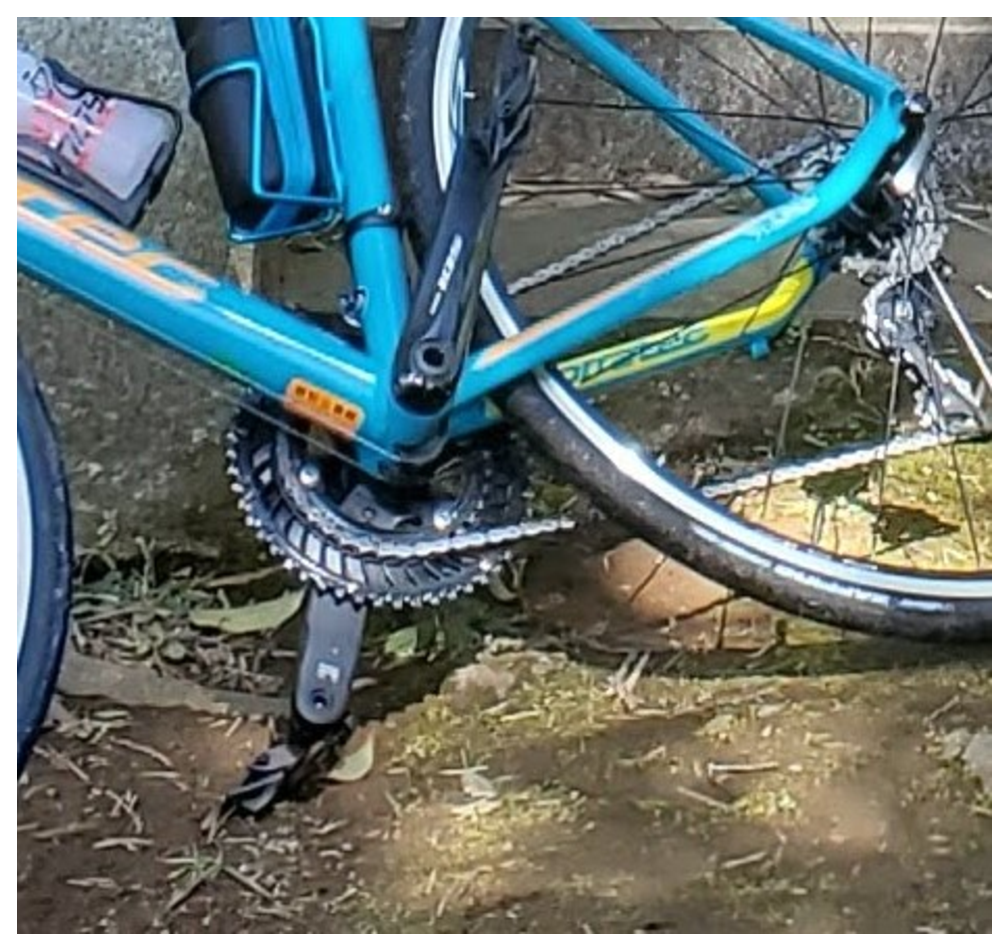
\includegraphics[clip,width = 9.0cm]{sample_cut.eps}
    \caption{DCT変換}
    \label{fig:sample}
    \end{figure}

\section{原理}
\subsection{JPEG}
JPEG(Joint Photographic Experts Group)とは,静止画像データを非可逆圧縮する方式の一種である.
この手法は次の2つの処理が行われる.
\begin{enumerate}
  \item 色情報の圧縮
  \item 空間周波数成分分析による圧縮
\end{enumerate}

まず一つ目の色情報の圧縮について説明する.
人の目は輝度と比較し,色の変化には弱い.この特性を利用し,$R$,$G$,$B$の各成分を輝度$Y$と色を表す$C_b$,$C_r$に変換する.
具体的には以下のように変換される.\cite{jpeg2}
\begin{equation}
  Y = 0.299R + 0.587G + 0.114B - 128
\end{equation}
\begin{equation}
  C_b = - 0.1687R - 0.3313G + 0.5B + 128
\end{equation}
\begin{equation}
  C_r = 0.5R - 0.4187G - 0.0813B + 128
\end{equation}
その後,ブロックごとに任意のピクセルを間引いてサンプリングを行うことで圧縮を行う.

次に,空間周波数成分分析による圧縮について説明する.
この手法では,元画像の各成分について,8×8画素ごとの小ブロックに分割し,各小ブロックについてDCT演算を行う.
DCT変換とは離散フーリエ変換の一種であり,cos波の重ね合わせで表現できることを応用した技術である.
DCTを実際に行った場合を図\ref{fig:dct}に示す.\cite{jpeg1}

\begin{figure}[htbp]
  \centering  % 図を真ん中に配置
  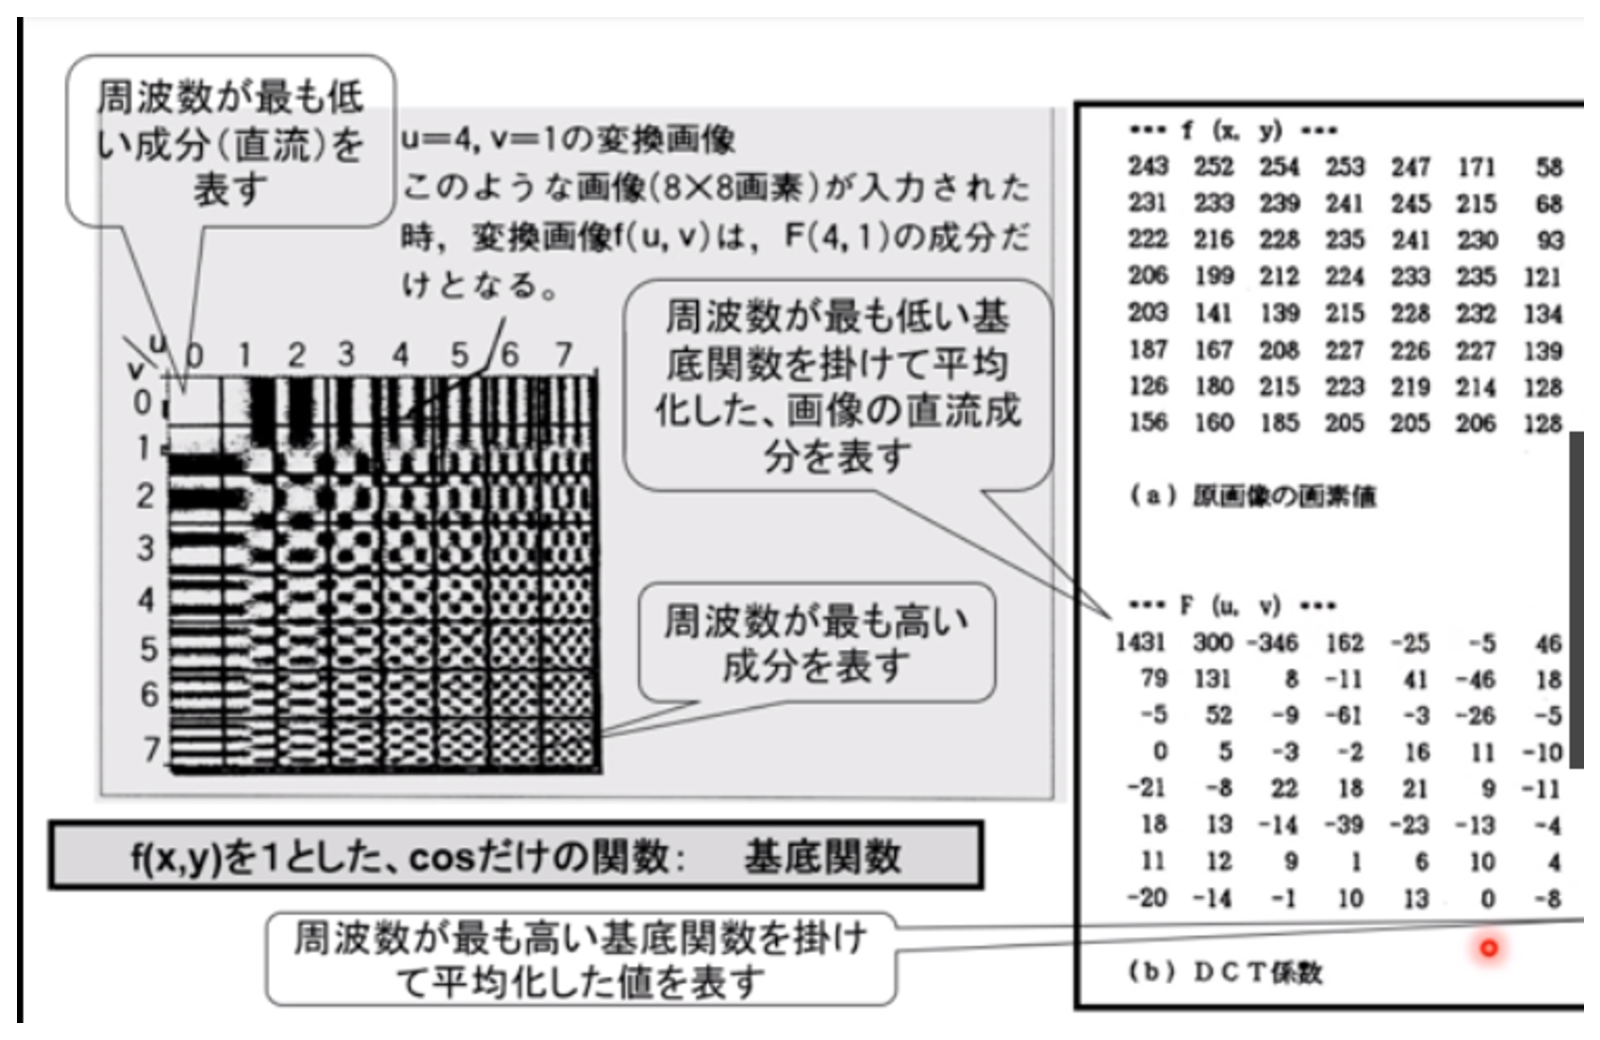
\includegraphics[clip,width = 12.0cm]{dct_con.eps}
  \caption{DCT変換}
  \label{fig:dct}
  \end{figure}

左上の方ほど空間周波数が低く,変化が少ない,その一方で右下の方ほど空間周波数が高い,変化が細かいことが確認できる.
周波数が高ければ高いほど細かなピクセルの変化を表すが,それらは間引いても違和感なく圧縮できる.



\subsection{PNG}
PNG(Portable Network Graphics)とは静止画像データを可逆圧縮する方式の一種である.
Webでビットマップ画像を扱うファイルフォーマットとして開発された.
理論上GIFよりも圧縮効率がよい。
また,Webのフォーマットように開発されたため,複数の透過色を指定可能,ガンマ値を補正できる特徴を持つ。
LZ77(正確にはLZSS)というアルゴリズムが使われており,GIFよりも圧縮率が高い.

 
\subsection{GIF}
GIFはPNGと同様に可逆圧縮をする方式である.1から256色と表現できる色が少なく,色を多く使用する写真などには向かないが、
イラストなど色が少ない場合は画像が軽量化されることがある,LWZというアルゴリズムが使われている.

%=====================================================================
\section{課題}
課題内容を以下に示す.

 \begin{enumerate}
    \item デジカメ等で撮影したJPEG画像の圧縮率を変化させて保存した複数の画像を作成し,画質とデータサイズとの関係を考察しなさい。また,画質がどのように変化しているか。またなぜそのような変化をするのかを考察しなさい。
    \item 同じ画像をJPEG以外の画像フォーマットで保存し,JPEGとの比較考察をしなさい。
  \end{enumerate}



\section{実験手順}
実験器具で示したスマートフォンと画像編集ソフトIrfanViewで実験を行った.
実験手順を以下に示す.\\

\begin{enumerate}
  \item \begin{enumerate}
          \item スマホで写真を撮影する.
          \item IrfanViewで写真を開く.
          \item "ファイル" → "名前をつけて保存"を選択する.
          \item ファイルの種類を"JPG-JPEG File"にする.
          \item "save options"より"save quality"(圧縮率)を10\textasciitilde100の20\%刻みで実行する.
        \end{enumerate}
  \item \begin{enumerate}
          \item ファイルの種類を"JPG-JPEG File"にする.
          \item "save options"より"save quality"(圧縮率)を10\textasciitilde100の79\%刻みで実行する.
          \item ファイルの種類を"PNG-Portable Network Graphics"にする.
          \item "save options"より"Compression level"(圧縮度)を1で実行する.
          \item ファイルの種類を"GIF-Compuserve GIF"にする.
          \item "save options"よりsave quality(圧縮率)を79\%で実行する.
        \end{enumerate}
\end{enumerate}

%=====================================================================
\section{結果}
  \subsection{課題1}
  圧縮率を10\textasciitilde100まで20\%刻みで行った.その結果を図\ref{fig:j10}\textasciitilde\ref{fig:j90}に示す.
  またそれぞれのファイルサイズは表\ref{tab:result_jpeg_filesize}のようになった.

  \begin{figure}[htbp]
    \begin{minipage}{0.5\hsize}
     \begin{center}
      \includegraphics[width=50mm]{sample_j10.jpg}
     \end{center}
     \caption{JPEG:圧縮率10\%}
     \label{fig:j10}
    \end{minipage}
    \begin{minipage}{0.5\hsize}
     \begin{center}
      \includegraphics[width=50mm]{sample_j30.jpg}
     \end{center}
     \caption{JPEG:圧縮率30\%}
     \label{fig:j30}
    \end{minipage}
   \end{figure}

   \begin{figure}[htbp]
    \begin{minipage}{0.5\hsize}
     \begin{center}
      \includegraphics[width=50mm]{sample_j50.jpg}
     \end{center}
     \caption{JPEG:圧縮率50\%}
     \label{fig:j50}
    \end{minipage}
    \begin{minipage}{0.5\hsize}
     \begin{center}
      \includegraphics[width=50mm]{sample_j70.jpg}
     \end{center}
     \caption{JPEG:圧縮率70\%}
     \label{fig:j70}
    \end{minipage}
   \end{figure}
\newpage
   \begin{figure}[htbp]
     \begin{center}
      \includegraphics[width=50mm]{sample_j90.jpg}
     \end{center}
     \caption{JPEG:圧縮率90\%}
     \label{fig:j90}
   \end{figure}

   \begin{table}[htb]
    \begin{center}
      \caption{JPEGで保存したときの画像サイズ一覧}
      \begin{tabular}{|c|c|} \hline
        圧縮率[\%] & サイズ[$kB$] \\\hline
        10 & 52  \\
        30 & 66  \\ 
        50 & 75  \\
        70 & 86  \\
        90 & 120  \\\hline

      \end{tabular}
      \label{tab:result_jpeg_filesize}
    \end{center}
  \end{table}
\newpage
  \subsection{課題2}
    条件をそろえるためPNGは圧縮レベル1を,GIFとJPEGは79\%に設定して圧縮を行った.
    その結果を図\ref{fig:j79}\textasciitilde\ref{fig:g79}に示す.

    \begin{figure}[htbp]
      \begin{minipage}{0.5\hsize}
       \begin{center}
        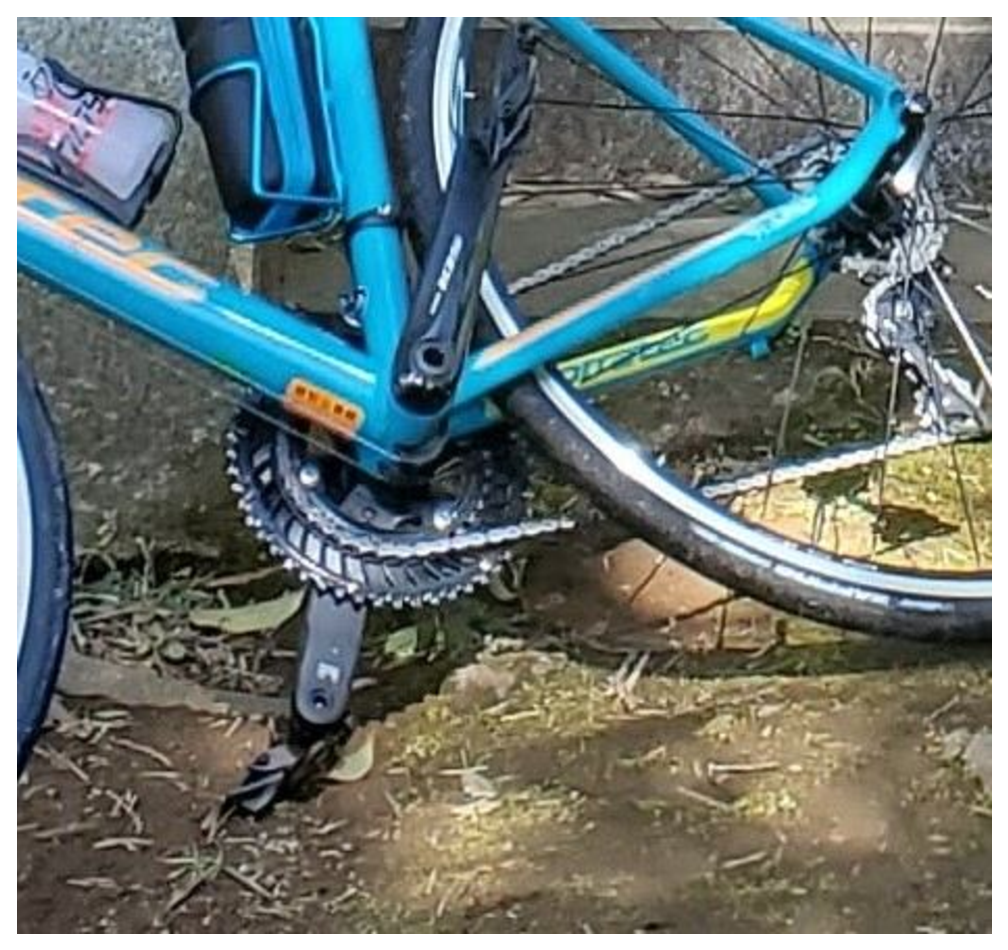
\includegraphics[width=50mm]{sample_j79.eps}
       \end{center}
       \caption{JPEG:圧縮率79\%}
       \label{fig:j79}
      \end{minipage}
      \begin{minipage}{0.5\hsize}
       \begin{center}
        \includegraphics[width=50mm]{sample_p79.eps}
       \end{center}
       \caption{PNG:圧縮率79\%}
       \label{fig:p79}
      \end{minipage}
     \end{figure}

     \begin{figure}[!htbp]
       \begin{center}
        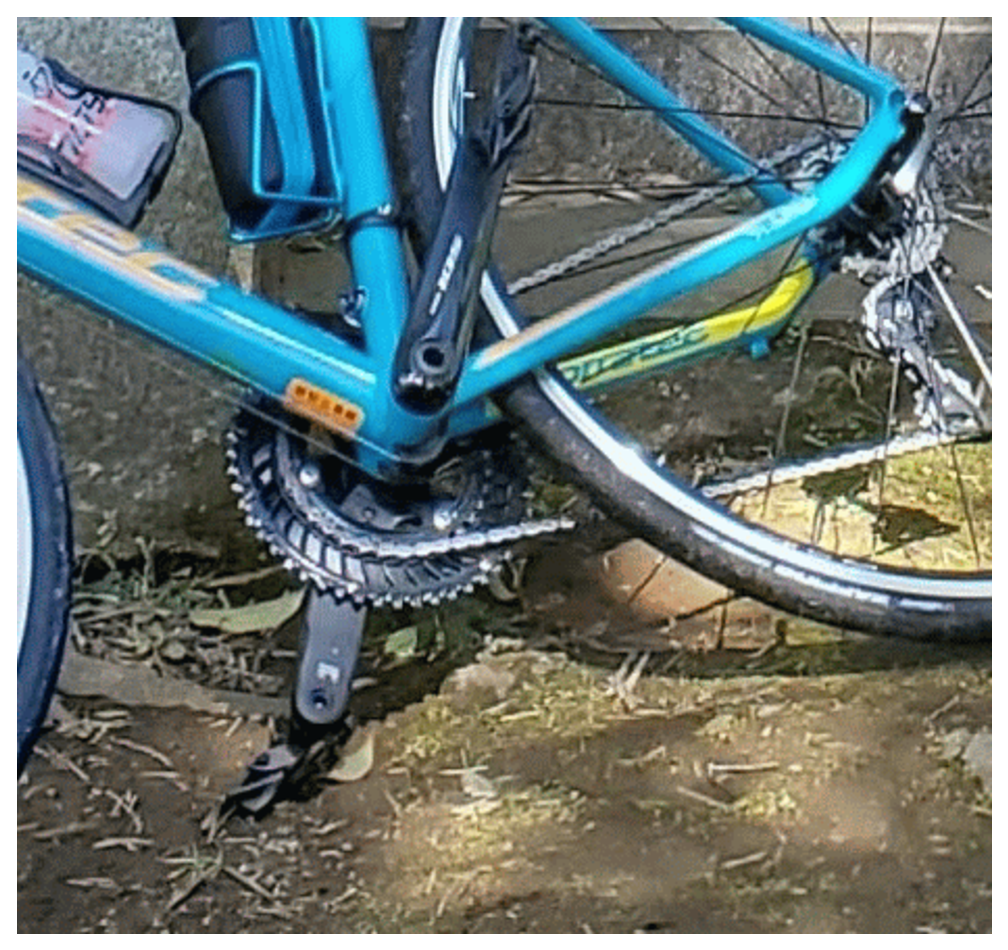
\includegraphics[width=50mm]{sample_g79.eps}
       \end{center}
       \caption{GIF:圧縮率79\%}
       \label{fig:g79}
     \end{figure}

     また,ファイルサイズは表\ref{tab:result_filesize}のようになった.
     \begin{table}[htb]
      \begin{center}
        \caption{圧縮率79\%の保存形式ごとのサイズ一覧}
        \begin{tabular}{|c|c|} \hline
          保存形式 & サイズ[$kB$] \\\hline
          JPEG & 94  \\
          PNG & 386  \\ 
          GIF & 154  \\ \hline

        \end{tabular}
        \label{tab:result_filesize}
      \end{center}
    \end{table}
  


   

\section{考察}
\subsection{課題1}

\subsection{課題2}
  高い圧縮率でJPEG圧縮をすると、8×8で圧縮処理を行う弊害として、以下の画像のように8×8のモザイク状のノイズ(ブロックノイズ)が生じてしまったり、高い空間周波数成分を間引いてしまったために、明るさや色が急激に変わる輪郭周辺でもやもやしたノイズ(モスキートノイズ)が現れたりすることがあります。
   また、圧縮するたびにデータの一部分が必ず劣化していきますので、画像処理を続けて行うときに、途中経過をJPEG形式で保存することはおすすめできません。
   少しでも画像劣化を避けたい場合、あるいは画像処理を続けて行う際の途中経過の保存などのためには、可逆圧縮方式を利用したPNGなどの別の形式を用いるか、データ量は少々多くなりますが圧縮しないでそのまま保存するなどの方法をとることがのぞましいです。


%=====================================================================
\section{参考文献}
\begin{thebibliography{99}
  \bibitem{jpeg1} 堀内 隆彦,マルチメディア工学Ⅰ第六回授業スライド(2020)
  \bibitem{jpeg2} しらぎくサイト,JPEG画像形式の概要(圧縮アルゴリズム),2004.9.20,https://www.marguerite.jp/Nihongo/Labo/Image/JPEG.html
\end{thebibliography}




\end{document}
